\documentclass{beamer}
% Required packages
\usepackage{amsmath}
\usepackage{physics}
\usepackage{graphicx}
\usepackage{siunitx}
\usepackage{xcolor}

% Set graphics path
\graphicspath{{../images/}}
% Define custom colors for DS9 theme
\definecolor{ds9blue}{RGB}{25,25,112}
\definecolor{ds9gold}{RGB}{218,165,32}
\definecolor{ds9grey}{RGB}{105,105,105}
\definecolor{ds9red}{RGB}{178,34,34}
% Set up the Madrid theme with custom colors
\usetheme{Madrid}
\usecolortheme{whale}
\setbeamercolor{palette primary}{bg=ds9blue,fg=white}
\setbeamercolor{palette secondary}{bg=ds9grey,fg=white}
\setbeamercolor{palette tertiary}{bg=ds9gold,fg=black}
\setbeamercolor{palette quaternary}{bg=ds9red,fg=white}
\setbeamercolor{structure}{fg=ds9blue}
\setbeamercolor{title}{fg=ds9gold}
\setbeamercolor{subtitle}{fg=ds9gold}
\setbeamercolor{frametitle}{bg=ds9blue,fg=white}
\setbeamercolor{block title}{bg=ds9blue,fg=white}
\setbeamercolor{block body}{bg=ds9grey!20,fg=black}

\title[Relative Velocity]{PHYS12 CH:3.5}
\subtitle{Addition of Velocities}
\author[Mr. Gullo]{Mr. Gullo}
\date[Sep 4, 2025]{September 4, 2025}

\begin{document}

\frame{\titlepage}

\begin{frame}{Outline}
    \tableofcontents
\end{frame}

\section{Introduction \& Objectives}

\begin{frame}{Learning Objectives}
    \begin{block}{By the end of this lesson, you will be able to:}
        \begin{itemize}
            \item Understand that velocity is measured relative to a specific frame of reference.
            \item Use subscript notation to represent and track relative velocities.
            \item Apply the principles of vector addition to solve 1D and 2D relative velocity problems.
        \end{itemize}
    \end{block}
\end{frame}

\section{Relative Velocity Principles}

\begin{frame}{What is Relative Velocity?}
    \begin{block}{Velocity Depends on Your Point of View}
        Imagine you are walking at \SI{1}{m/s} down the aisle of a train that is moving at \SI{10}{m/s}.
        \begin{itemize}
            \item To someone sitting on the train, your speed is \SI{1}{m/s}.
            \item To someone standing on the ground, your speed is \SI{1}{m/s} + \SI{10}{m/s} = \SI{11}{m/s}.
        \end{itemize}
        The velocity of an object depends on the \textbf{reference frame} from which it is measured. All velocity addition problems are vector addition problems.
    \end{block}
    
    \begin{center}
    \alert{[Diagram showing a train moving with vector $v_{train/ground}$ and a person walking with vector $v_{person/train}$. The resultant vector $v_{person/ground}$ is shown as their sum.]}
    \end{center}
\end{frame}

\begin{frame}{Relative Velocity Visualization}
    \begin{center}
    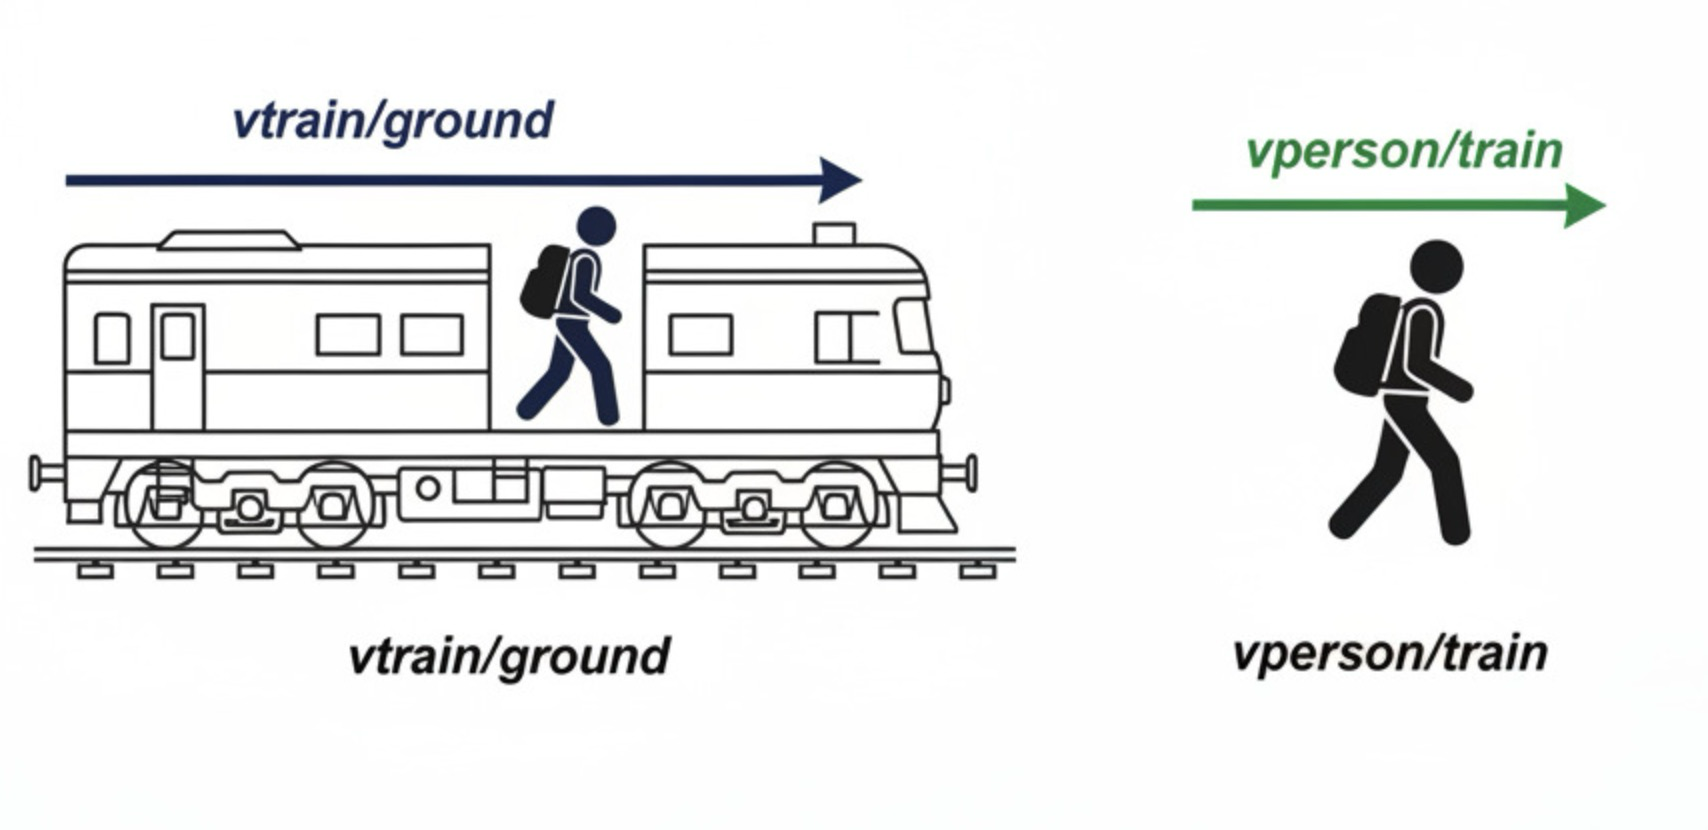
\includegraphics[width=0.8\linewidth]{phys12-relative-velocity-train.png}
    \end{center}
    
    \begin{block}{Understanding the Diagram}
        \begin{itemize}
            \item The train moves with velocity $\vb{v}_{train/ground}$ relative to the ground
            \item The person walks with velocity $\vb{v}_{person/train}$ relative to the train
            \item The person's velocity relative to the ground is the vector sum: $\vb{v}_{person/ground} = \vb{v}_{person/train} + \vb{v}_{train/ground}$
        \end{itemize}
    \end{block}
\end{frame}

\begin{frame}{The Relative Velocity Equation}
    \begin{block}{A "Chain Rule" for Velocities}
        We use subscripts to keep track of reference frames. The velocity of object A relative to frame C is the vector sum of A's velocity relative to B, and B's velocity relative to C.
        
        \Large{\[ \vb{v}_{AC} = \vb{v}_{AB} + \vb{v}_{BC} \]}
        
        \begin{itemize}
            \item The "inner" subscripts must match.
            \item The "outer" subscripts give the resultant vector.
        \end{itemize}
    \end{block}
    
    \begin{alertblock}{Important Relationship}
        The velocity of A relative to B is the negative of the velocity of B relative to A.
        \[ \vb{v}_{AB} = - \vb{v}_{BA} \]
    \end{alertblock}
\end{frame}

\section{Problem Solving Examples}

\begin{frame}{I do: 1D Headwind (Problem 52)}
    \begin{block}{Problem}
        Bryan Allen pedaled a human-powered aircraft for \SI{169}{min} at an average velocity of \SI{3.53}{m/s} in a direction \ang{45} south of east. During the flight, he encountered a headwind averaging \SI{2.00}{m/s} in the opposite direction of his motion.
        
        What was his average velocity relative to the air?
    \end{block}
    \begin{block}{Strategy}
        This is a 1D problem because the headwind is exactly opposite to the direction of motion. We only need to consider the magnitudes.
    \end{block}
\end{frame}

\begin{frame}{I do: 1D Headwind (Solution)}
    \begin{block}{Step 1: Define Frames and Equation}
        \begin{itemize}
            \item P = Plane (Bryan's aircraft)
            \item G = Ground (Earth)
            \item A = Air (the headwind)
        \end{itemize}
        The relationship is: $\vb{v}_{PG} = \vb{v}_{PA} + \vb{v}_{AG}$
        We want to find his speed relative to the air, $\vb{v}_{PA}$.
    \end{block}
    
    \begin{block}{Step 2: Rearrange and Solve}
        Rearrange the equation: $\vb{v}_{PA} = \vb{v}_{PG} - \vb{v}_{AG}$
        
        \begin{itemize}
            \item $\vb{v}_{PG}$ = \SI{3.53}{m/s} (velocity relative to the ground)
            \item $\vb{v}_{AG}$ = \SI{-2.00}{m/s} (wind velocity relative to ground; negative because it's a headwind, opposite to $\vb{v}_{PG}$)
        \end{itemize}
        
        $v_{PA} = (\SI{3.53}{m/s}) - (\SI{-2.00}{m/s}) = \SI{5.53}{m/s}$
        
        His speed relative to the air was \SI{5.53}{m/s}. He had to pedal this fast just to make \SI{3.53}{m/s} of progress over the ground.
    \end{block}
\end{frame}

\begin{frame}{We do: 2D Ship in a Current (Problem 57)}
    \begin{block}{Problem}
        A ship sets sail from Rotterdam, heading due north at \SI{7.00}{m/s} relative to the water. The local ocean current is \SI{1.50}{m/s} in a direction \ang{40.0} north of east.
        
        What is the velocity of the ship relative to the Earth?
    \end{block}
    
    \begin{center}
    \alert{[Diagram showing a vector pointing north for the ship's velocity relative to water, and a vector pointing 40 deg N of E for the current. The task is to find their vector sum.]}
    \end{center}
\end{frame}

\begin{frame}{We do: 2D Ship in a Current (Setup)}
    \begin{block}{Step 1: Define Frames and Equation}
        \begin{itemize}
            \item B = Boat
            \item W = Water (current)
            \item G = Ground (Earth)
        \end{itemize}
        We need to find $\vb{v}_{BG}$. The equation is: $\vb{v}_{BG} = \vb{v}_{BW} + \vb{v}_{WG}$
    \end{block}
    
    \begin{block}{Step 2: Find Components of Each Vector}
        Let's set up a component table. (East = +x, North = +y)
        \begin{itemize}
            \item Ship relative to Water ($\vb{v}_{BW}$): heads due north. \\
            $v_{BW,x} = 0$ \\
            $v_{BW,y} = +\SI{7.00}{m/s}$
            \item Water relative to Ground ($\vb{v}_{WG}$): current at \ang{40} N of E. \\
            $v_{WG,x} = (\SI{1.50}{m/s})\cos(\ang{40.0}) = +\SI{1.15}{m/s}$ \\
            $v_{WG,y} = (\SI{1.50}{m/s})\sin(\ang{40.0}) = +\SI{0.96}{m/s}$
        \end{itemize}
    \end{block}
    \end{frame}

\begin{frame}
    \begin{alertblock}{Step 3: Let's find the Resultant!}
        How do we find the x and y components of the ship's velocity relative to the ground ($\vb{v}_{BG}$)? How do we find its final speed and direction?
    \end{alertblock}
\end{frame}

\begin{frame}{You do: Finding the Wind Speed}
    \begin{block}{Problem}
        A seagull flies at a velocity of \SI{9.00}{m/s} straight into the wind. If it takes the bird \SI{20.0}{min} to travel \SI{6.00}{km} relative to the Earth, what is the velocity of the wind?
    \end{block}
    
    \begin{alertblock}{Hints}
        \begin{enumerate}
            \item Define your frames: S=Seagull, A=Air, G=Ground.
            \item First, calculate the seagull's velocity relative to the ground ($\vb{v}_{SG}$) from the distance and time data.
            \item You are given the seagull's speed relative to the air ($\vb{v}_{SA}$).
            \item Write the relative velocity equation and rearrange it to solve for the velocity of the wind ($\vb{v}_{AG}$).
        \end{enumerate}
    \end{alertblock}
\end{frame}

\section{Summary}

\begin{frame}{Summary}
    \begin{block}{Key Concepts for Relative Velocity}
        \begin{itemize}
            \item All velocity is relative to a reference frame.
            \item The key to solving problems is the vector equation:
            \[ \vb{v}_{AC} = \vb{v}_{AB} + \vb{v}_{BC} \]
            \item Always identify the reference frames (e.g., plane, air, ground) before you begin.
            \item 2D problems are solved by breaking each velocity vector into x and y components and then summing the components, just like any other vector addition problem.
        \end{itemize}
    \end{block}
\end{frame}

\end{document}